\section{Мета роботи}
Набути практичного досвіду та закріпити знання про подання
стека, дека, пріоритетної черги та дисципліни їх обслуговування.
\\

\noindent
\textbf{Теми для попередньої роботи:}
\begin{itemize}
    \item масиви та списки;
    \item безпріоритетні та пріоритетні черги;
    \item дисципліни обслуговування черг.
\end{itemize}



\section{Завдання}
Розробити функції, що забезпечують запис та читання запитів із пріоритетної черги, стека або дека.
В кожному завданні для організації вказаної черги використати дві структури.
Перевірити працездатність розроблених функцій.
Послідовність виконання операцій запису та читання обирати випадково.
Порівняти результати роботи, зробити висновки.
\\

\noindent
\textbf{Завдання за варіантом (\variant)}\\
Стек. Стек організований на двоспрямованому списку та на масиві
і «зростає» від меншої адреси пам’яті до більшої.



\section{Хід виконання}
Для виконання завдання було обрано мову Rust.
Увесь код також додатково був розміщений в GitHub репозитарії: \href{https://github.com/blackgolyb/algos-labs}{https://github.com/blackgolyb/algos-labs}.


\newpage
\subsection{Vector}
Для цього завдання напишемо власну реалізацю вектора яка буде використовуватися далі
\lstinputlisting[language=Rust, style=colouredRust]{\codeDirectory/src/libs/vector/lib.rs}

\newpage
\subsection{Linked List}
Для цього завдання напишемо власну реалізацю двозвязного списку яка буде використовуватися далі
\lstinputlisting[language=Rust, style=colouredRust]{\codeDirectory/src/libs/list/double_linked_list.rs}


\newpage
\subsection{Спільний інтерфейс для стека}
Для подальших імплементацій стека напишемо спільний інтерфейс
\lstinputlisting[language=Rust, style=colouredRust]{\codeDirectory/src/libs/stack/base.rs}

\newpage
\subsection{Стек на основі вектора}
\lstinputlisting[language=Rust, style=colouredRust]{\codeDirectory/src/libs/stack/vector_stack.rs}

\newpage
\subsection{Стек на основі списка}
\lstinputlisting[language=Rust, style=colouredRust]{\codeDirectory/src/libs/stack/list_stack.rs}

\newpage
\subsection{Приклад роботи програми}
Напишемо програму яка буде перевіряти та порівнювати скільки часу займає додавання та видалення елементів зі стека для обох варіантів
\noindent
Код програми для перевірки:
\lstinputlisting[language=Rust, style=colouredRust]{\codeDirectory/src/labs/lab7/main.rs}

\begin{figure}[ht!]
    \centering
    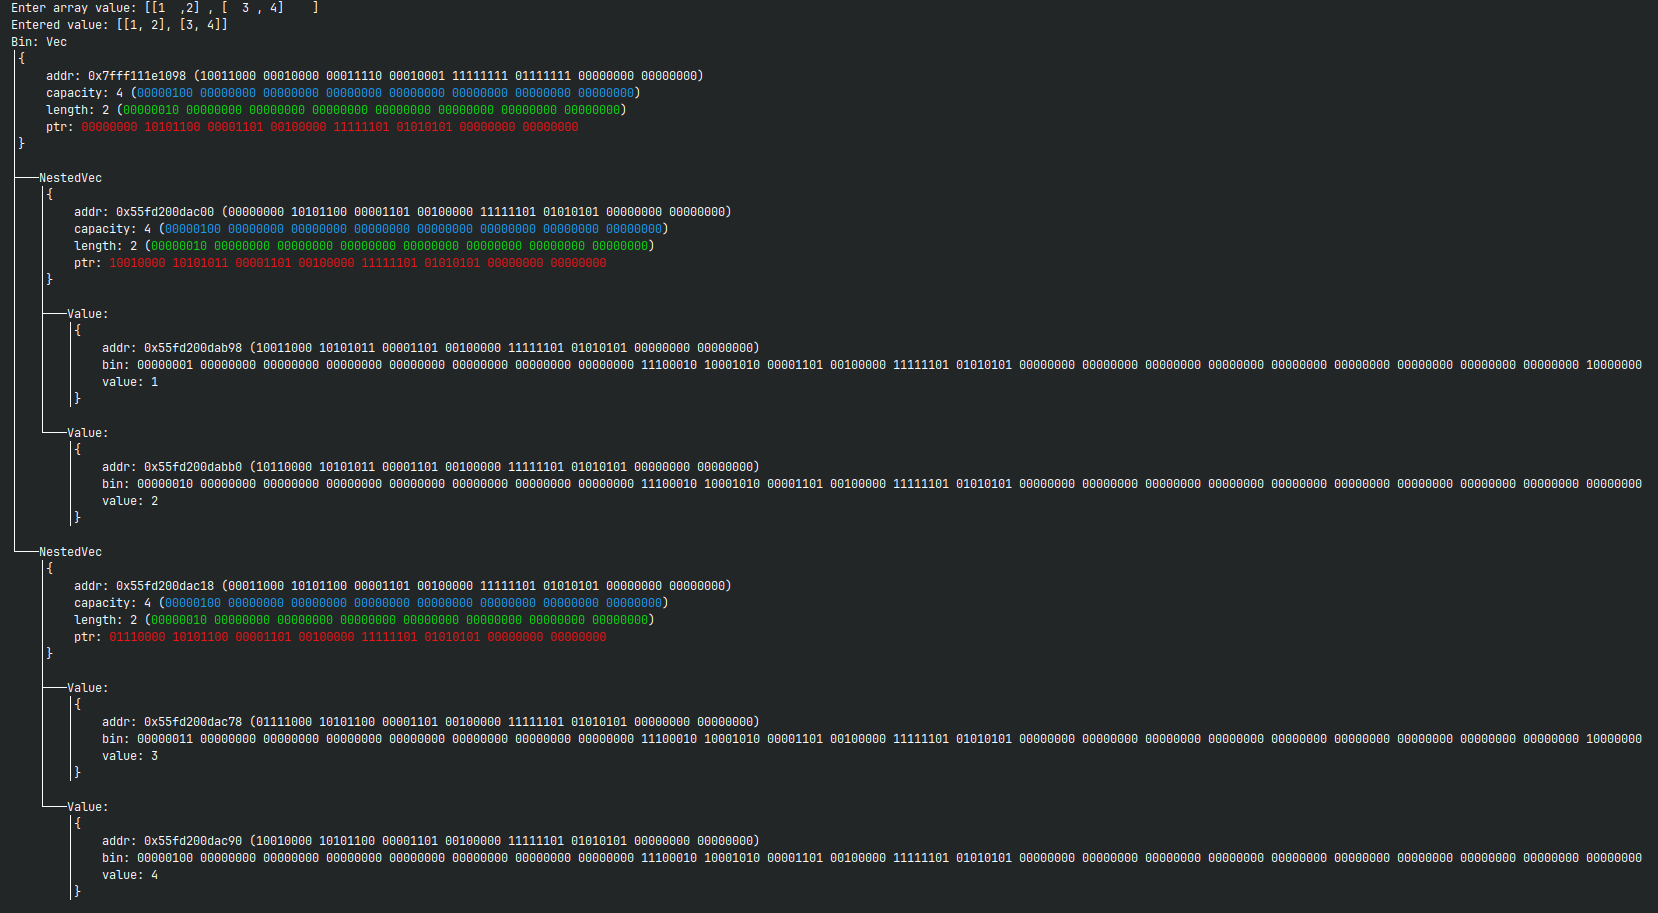
\includegraphics[width=.9\textwidth]{\assetsDirectory/res.png}
    \caption{Приклад роботи}
\end{figure}


\newpage
\section{Висновки}
В ході виконання лабораторної робити було створено 2 варіанти подання стека.
За результатами порівняння було виявлено, що стек на основі вектора є ефективнішим як за доданням, так і за видаленням.
Тому використання такого подання буде ефективнішим для більшості завдань.
Проте використання стека на основі списика може бути раціональним коли нам треба зберігати великий обсяг даних в елементах стека,
бо не треба виділяти неперервну ділянку пам'яті для цих елементів на відміну від векторного представлення.
